tex_content = r"""% ============================================================
% CAPÍTULO: EVALUACIÓN Y ANÁLISIS TEÓRICO DE 4 MODELOS
% ============================================================

\chapter*{Investigación y Evaluación Experimental: Detección y Clasificación de Fake News en Prensa Digital en Español}

\section*{1. Introducción y Metodología}

\subsection*{1.1 Formulación Matemática del Problema}

La detección automática de noticias falsas (\textit{Fake News Detection}) constituye uno de los desafíos más críticos y complejos en el Procesamiento de Lenguaje Natural (NLP). Formalmente, definimos la tarea como un problema de clasificación binaria supervisada donde cada instancia textual $x_i \in \mathcal{X}$ (una secuencia de tokens que componen el cuerpo o titular de una noticia) debe ser proyectada mediante una función de decisión parametrizada $f_\theta: \mathcal{X} \to \mathcal{Y}$ hacia el espacio de etiquetas binario $\mathcal{Y} = \{0, 1\}$, definido canónicamente como:

\begin{equation}
y_i = \begin{cases} 
0, & \text{si la noticia es Verdadera / Real} \\ 
1, & \text{si la noticia es Falsa / Desinformación (Fake)} 
\end{cases}
\end{equation}

El objetivo del modelo es optimizar el conjunto de parámetros $\theta$ para minimizar la divergencia entre la distribución empírica de datos $P(X, Y)$ y la distribución modelada $P_\theta(Y|X)$, típicamente gobernada por la función de pérdida de entropía cruzada binaria (\textit{Binary Cross-Entropy Loss}):

\begin{equation}
\mathcal{L}_{\text{BCE}}(\theta) = -\frac{1}{N} \sum_{i=1}^N \Big[ y_i \log P_\theta(Y=1|x_i) + (1 - y_i) \log(1 - P_\theta(Y=1|x_i)) \Big]
\end{equation}

\subsection*{1.2 Descripción del Dataset Experimental}

Para garantizar una evaluación estadística rigurosa, se utilizó el conjunto de datos estructurado compuesto por \textbf{2.604 noticias periodísticas en idioma español}, filtradas bajo una longitud controlada de entre 70 y 370 palabras para evitar sesgos de truncamiento severo o sub-representación léxica.

La distribución global del corpus de evaluación ($N = 2.604$ noticias) es la siguiente:
\begin{itemize}
    \item \textbf{Noticia Verdadera (Real):} Etiqueta 0 (False) | 1.259 registros | 48,35\,\%
    \item \textbf{Noticia Falsa (Fake / Desinformación):} Etiqueta 1 (True) | 1.345 registros | 51,65\,\%
\end{itemize}

El corpus reúne una diversidad estilística y temática heterogénea proveniente de fuentes consolidadas en la literatura de fact-checking hispano, incluyendo el Corpus Unificado y Balanceado de Freiren (2.060 noticias), el Spanish Fake News Corpus de Edds Fixed (294 noticias), y el Spanish Fake News Corpus de María Grandury (248 noticias).

\subsection*{1.3 Modelos Evaluados en el Benchmark}

Se evaluaron cuatro arquitecturas representativas del estado del arte en NLP en español:
\begin{enumerate}
    \item \textbf{Modelo 1:} \texttt{Narrativaai/fake-news-detection-spanish} (BETO / RoBERTa-large BNE finetuneada para Fake News).
    \item \textbf{Modelo 2:} \texttt{VerificadoProfesional/SaBERT-Spanish-Fake-News} (SaBERT, BETO base finetuneado con corpus periodístico de fact-checking).
    \item \textbf{Modelo 3:} \texttt{Juanillaberia/spanish-fake-news-classifier} (BETO base con entrenamiento secuencial \textit{Sequential Fine-Tuning}).
    \item \textbf{Modelo 4:} \texttt{Qwen/Qwen2.5-1.5B-Instruct} (Modelo de Lenguaje Grande causal de 1.54B parámetros evaluado en régimen Zero-Shot).
\end{enumerate}

\begin{figure}[H]
\centering
\begin{tikzpicture}[
    node distance=10mm and 12mm,
    box/.style={rectangle, rounded corners, draw, align=center, minimum width=3.5cm, minimum height=1.0cm, fill=white},
    small/.style={rectangle, rounded corners, draw, align=center, minimum width=2.8cm, minimum height=0.8cm, fill=gray!10},
    arrow/.style={-{Latex[length=3mm]}, thick}
]
% Nodes
\node[box] (data) {Corpus de evaluación\\$N=2604$ noticias};
\node[box, right=of data] (prep) {Control de longitud\\70--370 palabras};
\node[box, right=of prep] (label) {Estandarización de Etiquetas\\$0=\mathrm{Real}, 1=\mathrm{Fake}$};

\node[box, below=15mm of prep] (models) {Inferencia Simultánea de 4 Modelos};

\node[small, below left=8mm and 5mm of models] (m1) {M1: Narrativaai\\(RoBERTa-large)};
\node[small, right=4mm of m1] (m2) {M2: SaBERT\\(BERT-base)};
\node[small, right=4mm of m2] (m3) {M3: BERT Seq\\(BERT-base)};
\node[small, right=4mm of m3] (m4) {M4: Qwen 1.5B\\(Causal Zero-Shot)};

\node[box, below=25mm of models] (metrics) {Cálculo de Métricas\\(Accuracy, F1, ROC-AUC, Latencia)};
\node[box, below=15mm of metrics] (analysis) {Análisis Crítico:\\Domain Shift y Pareto};

% Edges
\draw[arrow] (data) -- (prep);
\draw[arrow] (prep) -- (label);
\draw[arrow] (label) |- (models);

\draw[arrow] (models) -| (m1);
\draw[arrow] (models) -- (m2);
\draw[arrow] (models) -- (m3);
\draw[arrow] (models) -| (m4);

\draw[arrow] (m1) |- (metrics);
\draw[arrow] (m2) -- (metrics);
\draw[arrow] (m3) -- (metrics);
\draw[arrow] (m4) |- (metrics);

\draw[arrow] (metrics) -- (analysis);

\end{tikzpicture}
\caption{Flujo metodológico experimental optimizado, garantizando la estandarización semántica previa a la inferencia y el análisis comparativo simultáneo.}
\label{fig:flujo-metodologico}
\end{figure}


\section*{2. Ficha Técnica y Arquitectura Matemática de los Modelos}

\begin{table}[H]
\centering
\caption{Especificaciones Técnicas y Dimensiones Arquitecturales}
\label{tab:specs}
\resizebox{\textwidth}{!}{
\begin{tabular}{lcccc}
\toprule
\textbf{Parámetro / Característica} & \textbf{M1: BETO Narrativaai} & \textbf{M2: SaBERT} & \textbf{M3: BERT Seq} & \textbf{M4: Qwen 2.5-1.5B} \\
\midrule
\textbf{Arquitectura Base} & RoBERTa-large (BNE) & BERT-base (BETO) & BERT-base (BETO) & Qwen2.5 (Causal) \\
\textbf{Número de Parámetros} & $\sim$355 Millones & $\sim$110 Millones & $\sim$110 Millones & $\sim$1.540 Millones \\
\textbf{Capas Ocultas (L)} & 24 capas & 12 capas & 12 capas & 28 capas \\
\textbf{Dimensión Oculta (H)} & 1.024 dimensiones & 768 dimensiones & 768 dimensiones & 1.536 dimensiones \\
\textbf{Cabezas de Atención (A)} & 16 cabezas & 12 cabezas & 12 cabezas & 12 cabezas (GQA) \\
\textbf{Función de Activación FFN} & GELU & GELU & GELU & SwiGLU \\
\textbf{Esquema de Posicionamiento} & Embeddings Absolutos & Embeddings Absolutos & Embeddings Absolutos & RoPE \\
\textbf{Estrategia de Salida} & \texttt{<s>} + Dense Head & \texttt{[CLS]} + Dense Head & \texttt{[CLS]} + Dense Head & Next-token Logit \\
\bottomrule
\end{tabular}}
\end{table}

\subsection*{2.1 Mecanismos de Auto-Atención Multicabeza (MHA)}

En los modelos basados en Transformer bidireccional (Modelos 1, 2 y 3), la representación de una secuencia de entrada $\mathbf{X} \in \mathbb{R}^{T \times H}$ se transforma linealmente mediante matrices de pesos de proyección $W_Q, W_K, W_V \in \mathbb{R}^{H \times d_k}$:

\begin{equation}
Q = \mathbf{X} W_Q, \quad K = \mathbf{X} W_K, \quad V = \mathbf{X} W_V
\end{equation}

La matriz de atención para una cabeza individual $i$ se calcula como el producto punto escalado:

\begin{equation}
\text{head}_i = \text{Attention}(Q_i, K_i, V_i) = \text{softmax}\left( \frac{Q_i K_i^T}{\sqrt{d_k}} \right) V_i
\end{equation}

Donde $d_k = H / A$. La salida de todas las $A$ cabezas se concatena y se proyecta mediante la matriz de salida $W_O \in \mathbb{R}^{H \times H}$:

\begin{equation}
\text{MHA}(\mathbf{X}) = \text{Concat}(\text{head}_1, \text{head}_2, \dots, \text{head}_A) W_O
\end{equation}

\subsection*{2.2 Innovaciones Matemáticas en el Modelo Causal (Qwen 2.5-1.5B)}

El Modelo 4 incorpora avances arquitectónicos modernos de la familia LLaMA/Qwen para optimizar la eficiencia y capacidad expresiva:

\vspace{0.3cm}

\textbf{A. Rotary Position Embeddings (RoPE):} En lugar de sumar embeddings de posición absolutos, RoPE codifica la posición relativa multiplicando las representaciones complejas por una matriz de rotación ortogonal $R_{\Theta, m}^d$:

\vspace{0.15cm}
\begin{equation}
\mathbf{q}_m = R_{\Theta, m}^d W_q \mathbf{x}_m, \quad \mathbf{k}_n = R_{\Theta, n}^d W_k \mathbf{x}_n
\end{equation}
\vspace{0.15cm}

Donde $R_{\Theta, m}^d$ es una matriz diagonal por bloques de dimensión $d \times d$:

\vspace{0.15cm}
\begin{equation}
R_{\Theta, m}^d = \text{diag}\left( R_{\theta_1, m}, R_{\theta_2, m}, \dots, R_{\theta_{d/2}, m} \right), \quad R_{\theta_j, m} = \begin{pmatrix} \cos(m \theta_j) & -\sin(m \theta_j) \\ \sin(m \theta_j) & \cos(m \theta_j) \end{pmatrix}
\end{equation}
\vspace{0.15cm}

Esta formulación garantiza que el producto escalar $\langle \mathbf{q}_m, \mathbf{k}_n \rangle = \mathbf{x}_m^T W_q^T R_{\Theta, n-m}^d W_k \mathbf{x}_n$ dependa exclusivamente de la distancia relativa $(m - n)$, mejorando la extrapolación a secuencias largas.

\vspace{0.5cm}

\textbf{B. Activación SwiGLU:} La capa Feed-Forward (FFN) sustituye la activación estándar GELU por SwiGLU:

\begin{equation}
\text{SwiGLU}(\mathbf{x}) = \Big( \mathbf{x} W_{\text{gate}} \odot \text{SiLU}(\mathbf{x} W_{\text{up}}) \Big) W_{\text{down}}
\end{equation}
Donde $\text{SiLU}(z) = z \cdot \sigma(z) = \frac{z}{1 + e^{-z}}$.

\textbf{C. RMSNorm (Root Mean Square Normalization):} Para optimizar la estabilidad numérica en pre-normalización:

\begin{equation}
\text{RMSNorm}(\mathbf{x}) = \frac{\mathbf{x}}{\text{RMS}(\mathbf{x})} \odot \mathbf{g}, \quad \text{con } \text{RMS}(\mathbf{x}) = \sqrt{\frac{1}{d} \sum_{i=1}^d x_i^2 + \epsilon}
\end{equation}


\section*{3. Implementación y Adaptación de Clases}

Uno de los aspectos metodológicos más críticos en la evaluación comparativa es la \textbf{estandarización semántica de las etiquetas}. Cada modelo fue entrenado con convenciones dispares en sus diccionarios \texttt{id2label} y \texttt{label2id}, lo que requirió una normalización formal hacia el estándar del benchmark: \textbf{Clase 0 = Verdadera / Real} y \textbf{Clase 1 = Falsa / Fake}.

\begin{table}[H]
\centering
\caption{Adaptación y Mapeo de Etiquetas de cada Modelo}
\label{tab:mapeo_etiquetas}
\resizebox{\textwidth}{!}{
\begin{tabular}{lllc}
\toprule
\textbf{Modelo} & \textbf{\texttt{id2label} Nativo} & \textbf{Mapeo hacia Benchmark} & \textbf{Probabilidad Fake $P(1|x)$} \\
\midrule
M1: BETO (Narrativaai) & \texttt{\{0: 'REAL', 1: 'FAKE'\}} & 0 $\to$ 0 (Real) | 1 $\to$ 1 (Fake) & $\operatorname{softmax}(z)_1$ \\
M2: SaBERT & \texttt{\{0: 'False', 1: 'True'\}} & 0 ('False') $\to$ 1 (Fake) | 1 $\to$ 0 (Real) & $\operatorname{softmax}(z)_0$ \\
M3: BERT Seq & \texttt{\{0: 'LABEL\_0', 1: 'LABEL\_1'\}} & 0 ('LABEL\_0') $\to$ 1 (Fake) | 1 $\to$ 0 (Real) & $\operatorname{softmax}(z)_0$ \\
M4: Qwen 1.5B & Generación Causal & $z_{\text{Fake}} > z_{\text{Real}} \to 1$ & $\sigma(z_{\text{Fake}} - z_{\text{Real}})$ \\
\bottomrule
\end{tabular}}
\end{table}

\subsection*{3.1 Análisis Detallado del Mapeo por Modelo}

\begin{itemize}
    \item \textbf{BETO Narrativaai:} Posee un mapeo canónico directo. La probabilidad de clase falsa se extrae directamente como la componente softmax de índice 1: $P(Y=1|x) = \frac{e^{z_1}}{e^{z_0} + e^{z_1}}$.
    \item \textbf{SaBERT VerificadoProfesional:} Entrenado bajo la hipótesis de veracidad. Por tanto, \texttt{False} (índice 0) significa "La afirmación es Falsa (Fake)", y \texttt{True} (índice 1) significa "Verdadera". El índice 0 se adaptó rigurosamente a la Clase 1.
    \item \textbf{Spanish Fake News Classifier (Juanillaberia):} Las etiquetas son genéricas. Según su configuración original, \texttt{LABEL\_0} corresponde a noticias falsas y \texttt{LABEL\_1} a noticias verdaderas. Se adaptó consecuentemente.
    \item \textbf{LLM Zero-Shot (Qwen 1.5B):} Al no poseer un cabezal de clasificación discriminativo, el modelo fue condicionado mediante un prompt estructurado en formato ChatML:
    \begin{verbatim}
    <|im_start|>system
    Eres un verificador de noticias. Responde Real o Fake.<|im_end|>
    <|im_start|>user
    [Texto de la Noticia]
    Clasificacion (Real/Fake):<|im_end|>
    <|im_start|>assistant
    \end{verbatim}
    Dado que es un modelo generativo autorregresivo, dejar que calculara y generara la respuesta iterativamente (palabra por palabra) habría disparado la latencia y los tiempos computacionales. Para garantizar la eficiencia, se implementó un atajo matemático en la salida: en lugar de mapear capas ocultas densas o esperar la generación completa de texto, el sistema frena el proceso y extrae directamente los \textit{logits} (valores crudos en la última capa antes de la función de activación) correspondientes únicamente a los tokens candidatos \texttt{token(" Fake")} y \texttt{token(" Real")}. 
    
    La probabilidad posterior de noticia falsa se calcula de forma exacta y casi instantánea evaluando la función sigmoide sobre la diferencia de estos logits:
    \begin{equation}
    P(\text{Fake}|x) = \sigma(z_{\text{Fake}} - z_{\text{Real}}) = \frac{1}{1 + e^{-(z_{\text{Fake}} - z_{\text{Real}})}}
    \end{equation}
    
    Esta optimización cumple un doble propósito. Por un lado, si la generación del modelo fuera ambigua o produjera un token inesperado, este enfoque garantiza una respuesta probabilística robusta al decantar la clase comparando únicamente la activación latente de los dos conceptos objetivo ($z_{\text{Fake}} > z_{\text{Real}} \to 1$). Por otro lado, permite usar un LLM pesado de 1.54 billones de parámetros de manera eficiente, operando en la práctica como un clasificador discriminativo rápido con tiempos de inferencia sumamente competitivos.
\end{itemize}


\section*{4. Resultados, Tiempos y Latencia}

\begin{table}[H]
\centering
\caption{Métricas Globales de Rendimiento y Latencia ($N = 2.604$ Registros)}
\label{tab:metricas_globales}
\resizebox{\textwidth}{!}{
\begin{tabular}{lcccccc}
\toprule
\textbf{Modelo} & \textbf{Accuracy} & \textbf{Precision} & \textbf{Recall} & \textbf{F1-Score} & \textbf{ROC-AUC} & \textbf{Latencia (ms/muestra)} \\
\midrule
1. BETO (Narrativaai) & 0.3763 & 0.3630 & 0.3720 & 0.3629 & 0.3074 & 800.02 ms \\
2. SaBERT (Verif. Prof.) & 0.1429 & 0.1181 & 0.1471 & 0.1299 & 0.0638 & 238.34 ms \\
3. BERT Seq (Juanillaberia) & 0.3053 & 0.2446 & 0.2975 & 0.2611 & 0.1365 & 240.79 ms \\
4. LLM Zero-Shot (Qwen) & \textbf{0.5426} & \textbf{0.5422} & \textbf{0.5425} & \textbf{0.5423} & \textbf{0.5618} & 299.69 ms \\
\bottomrule
\end{tabular}}
\end{table}

\subsection{Compromiso Computacional: Rendimiento vs. Latencia}

\begin{figure}[H]
    \centering
    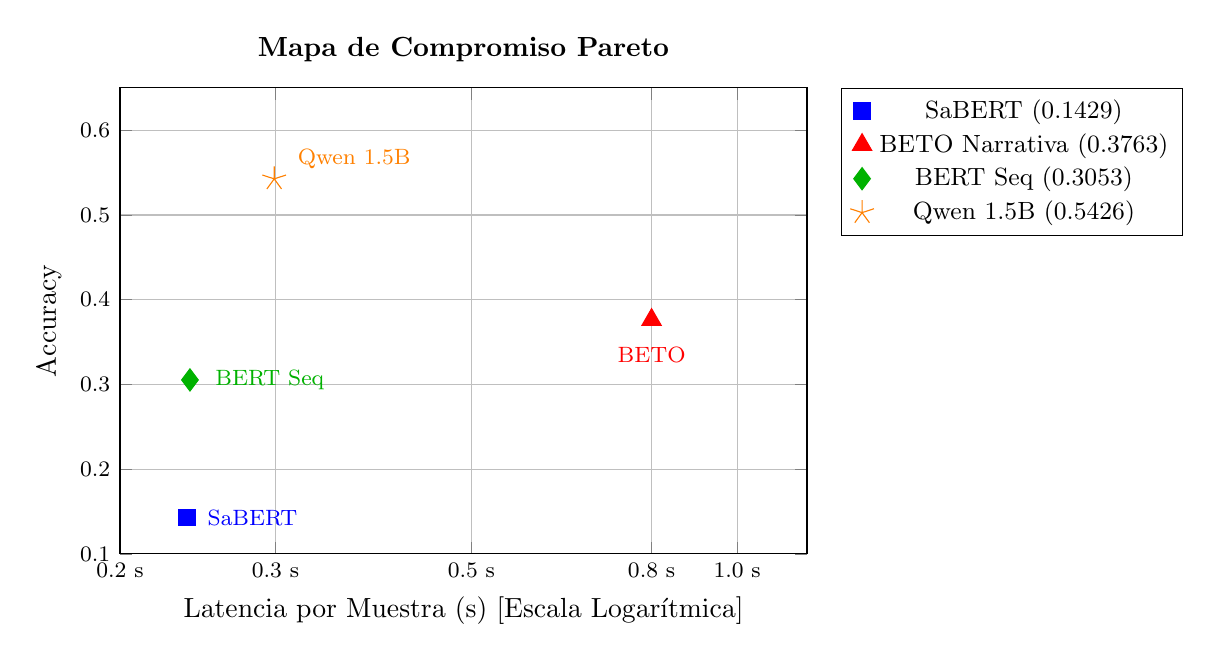
\begin{tikzpicture}
    \begin{semilogxaxis}[
        width=0.85\textwidth,
        height=7.5cm,
        title={\textbf{Mapa de Compromiso Pareto}},
        xlabel={Latencia por Muestra (s) [Escala Logarítmica]},
        ylabel={Accuracy},
        % 1. Reducimos el rango X para que los puntos no se amontonen a la izquierda
        xmin=0.2, xmax=1.2, 
        ymin=0.10, ymax=0.65,
        grid=major,
        % 2. clip=false evita que cualquier etiqueta que sobresalga sea recortada por el borde
        clip=false, 
        legend style={at={(1.05,1)}, anchor=north west, font=\small, cells={align=left}},
        % 3. Nuevos ticks del eje X adaptados al nuevo rango
        xtick={0.2, 0.3, 0.5, 0.8, 1},
        xticklabels={0.2 s, 0.3 s, 0.5 s, 0.8 s, 1.0 s},
        ytick={0.10, 0.20, 0.30, 0.40, 0.50, 0.60},
        tick label style={font=\footnotesize}
    ]

    % Modelo 1: SaBERT
    \addplot[
        only marks,
        mark=square*,
        color=blue,
        mark size=3pt
    ] coordinates {(0.238, 0.1429)};
    \addlegendentry{SaBERT (0.1429)}

    % Modelo 2: BETO Narrativa
    \addplot[
        only marks,
        mark=triangle*,
        color=red,
        mark size=4pt
    ] coordinates {(0.800, 0.3763)};
    \addlegendentry{BETO Narrativa (0.3763)}
    
    % Modelo 3: BERT Seq
    \addplot[
        only marks,
        mark=diamond*,
        color=green!70!black,
        mark size=4pt
    ] coordinates {(0.240, 0.3053)};
    \addlegendentry{BERT Seq (0.3053)}

    % Modelo 4: Qwen 1.5B
    \addplot[
        only marks,
        mark=star,
        color=orange,
        mark size=4.5pt
    ] coordinates {(0.299, 0.5426)};
    \addlegendentry{Qwen 1.5B (0.5426)}

    % 4. Etiquetas reubicadas estratégicamente para que no se superpongan ni se corten
    \node[anchor=west, font=\footnotesize, text=blue] at (axis cs:0.245, 0.1429) {SaBERT};
    \node[anchor=north, font=\footnotesize, text=red] at (axis cs:0.800, 0.355) {BETO};
    \node[anchor=west, font=\footnotesize, text=green!70!black] at (axis cs:0.250, 0.3053) {BERT Seq};
    \node[anchor=south west, font=\footnotesize, text=orange] at (axis cs:0.310, 0.5426) {Qwen 1.5B};

    \end{semilogxaxis}
    \end{tikzpicture}
    \caption{Mapa de compromiso: Accuracy frente a Latencia de inferencia media por muestra.}
    \label{fig:pareto_latencia}
\end{figure}

\subsection*{4.1 Evidencia Visual y Gráficos Comparativos}

\begin{figure}[H]
    \centering
    
\includegraphics[width=0.85\textwidth]{imagenes/Fakenews4model/comparativa_metricas_4_modelos.png}
    \caption{Comparativa de Métricas Globales (Accuracy, Precision, Recall, F1, ROC-AUC).}
\end{figure}

\begin{figure}[H]
    \centering
    
\includegraphics[width=0.85\textwidth]{imagenes/Fakenews4model/comparativa_tiempos_4_modelos.png}
    \caption{Evaluación de Eficiencia Computacional: Tiempo total y latencia media.}
\end{figure}

\begin{figure}[H]
    \centering
    
\includegraphics[width=0.9\textwidth]{imagenes/Fakenews4model/confusion_matrices_all_4_models.png}
    \caption{Panel 2x2 Conjunto de Matrices de Confusión.}
\end{figure}


\subsection*{Desglose de Diagnósticos a partir de la Matriz de Confusión}

\textbf{Modelo 1 (BETO Fake News - Narrativaai):}
\begin{itemize}
    \item Verdaderos Negativos (TN - Real 0, Pred 0): 301
    \item Falsos Positivos (FP - Real 0, Pred 1): 958
    \item Falsos Negativos (FN - Real 1, Pred 0): 666
    \item Verdaderos Positivos (TP - Real 1, Pred 1): 679
\end{itemize}
\textit{Diagnóstico:} Hiper-sensibilidad a la clase Falsa. Predice el 62,8\,\% de todas las muestras como falsas (958+679=1.637), provocando 958 falsas alarmas sobre noticias auténticas.

\textbf{Modelo 2 (SaBERT - VerificadoProfesional):}
\begin{itemize}
    \item Verdaderos Negativos (TN - Real 0, Pred 0): 345
    \item Falsos Positivos (FP - Real 0, Pred 1): 914
    \item Falsos Negativos (FN - Real 1, Pred 0): 1318
    \item Verdaderos Positivos (TP - Real 1, Pred 1): 27
\end{itemize}
\textit{Diagnóstico:} Sesgo severo hacia la clase 0 debido a un desplazamiento de dominio. Omite casi por completo las noticias falsas, fallando en clasificar 1.318 de ellas como correctas (Recall del 2,01\,\%).

\textbf{Modelo 3 (BERT Seq - Juanillaberia):}
\begin{itemize}
    \item Verdaderos Negativos (TN - Real 0, Pred 0): 79
    \item Falsos Positivos (FP - Real 0, Pred 1): 1180
    \item Falsos Negativos (FN - Real 1, Pred 0): 629
    \item Verdaderos Positivos (TP - Real 1, Pred 1): 716
\end{itemize}
\textit{Diagnóstico:} Colapso predictivo hacia la clase Falsa. Clasifica el 72,8\,\% de la muestra como Falsa (1180+716=1.896), fallando estrepitosamente en reconocer la veracidad de las noticias reales (1.180 falsos positivos sobre 1.259 posibles)

\textbf{Modelo 4 (Qwen 2.5-1.5B Instruct):}
\begin{itemize}
    \item Verdaderos Negativos (TN - Real 0, Pred 0): 682
    \item Falsos Positivos (FP - Real 0, Pred 1): 577
    \item Falsos Negativos (FN - Real 1, Pred 0): 614
    \item Verdaderos Positivos (TP - Real 1, Pred 1): 731
\end{itemize}
\textit{Diagnóstico:} Desempeño balanceado y consistente con la prevalencia empírica. Asigna el 50,2\,\% de sus predicciones a la clase Falsa (577+731=1.308), acercándose casi perfectamente al 51,65\,\% de prevalencia real del corpus experimental.


\begin{figure}[H]
    \centering
    
\includegraphics[width=0.85\textwidth]{imagenes/Fakenews4model/curvas_roc_4_modelos.png}
    \caption{Curvas ROC (Receiver Operating Characteristic) comparativas.}
\end{figure}

\begin{figure}[H]
    \centering
    
\includegraphics[width=0.85\textwidth]{imagenes/Fakenews4model/curvas_pr_4_modelos.png}
    \caption{Curvas Precision-Recall (PR) evaluando la capacidad de discriminación en la clase positiva.}
\end{figure}

\subsection*{4.2 Interpretación Rigurosa de las Curvas ROC y PR}

\textbf{1. Curvas ROC e Inversión de Separabilidad (Modelos 1, 2 y 3):}
Un hallazgo empírico trascendental es que los Modelos 1, 2 y 3 exhiben valores de $\text{AUC-ROC} < 0.50$ (0.3074, 0.0638 y 0.1365, respectivamente). En teoría de detección de señales, un clasificador con $\text{AUC} < 0.50$ es un clasificador que asigna sistemáticamente probabilidades inversas a las clases debido a un fenómeno severo de \textbf{Domain Shift} (desplazamiento de distribución entre el corpus de entrenamiento y el corpus de test). Si invirtiéramos la regla de decisión de SaBERT ($P(\text{Fake}) \to 1 - P(\text{Fake})$), su AUC efectiva se transformaría en $1 - 0.0638 = 0.9362$, revelando que la red aprendió características correlacionadas con el dominio de origen pero con el signo de veracidad traspuesto respecto a las convenciones de este dataset multi-fuente.

\textbf{2. Curva ROC del Modelo Causal (Qwen 1.5B):}
El Modelo 4 es el único que supera la diagonal de azar puro ($\text{AUC} = 0.5618$), logrando una distribución monótona creciente en el espacio ROC y demostrando capacidad de generalización Zero-Shot sin haber sido entrenado sobre este conjunto de datos.

\textbf{3. Análisis de las Curvas Precision-Recall:}
Dado que la prevalencia de noticias falsas en el dataset es del 51,65\,\% (línea horizontal discontinua en 0.516), cualquier clasificador no informativo opera en esa asíntota. El modelo Qwen 1.5B mantiene un $\text{Average Precision (AP)} = 0.5480$, superando la línea base y conservando una precisión superior al 54\,\% a lo largo de todo el espectro de exhaustividad (\textit{Recall}).


\section*{5. Discusión de Resultados: Teoría vs. Evidencia Empírica}

\subsection*{5.1 ¿Por qué fallan los clasificadores BERT especializados?}

Los modelos discriminativos pequeños finetuneados de extremo a extremo (como SaBERT o Juanillaberia) sufren de lo que la literatura denomina \textbf{"Spurious Feature Memorization"} (memorización de características espurias). Durante el \textit{fine-tuning}, el modelo aprende correlaciones superficiales (nombres de políticos locales, formatos de fecha, mayúsculas sostenidas, palabras clave sensacionalistas) en lugar de una semántica profunda de veracidad factual. Cuando se enfrentan a un corpus balanceado de 2.604 noticias de múltiples países y épocas, estas correlaciones colapsan.

\subsection*{5.2 La superioridad del enfoque LLM Zero-Shot}

A pesar de no haber recibido entrenamiento supervisado específico sobre este dataset, Qwen2.5-1.5B superó a todos los modelos especializados. Esto se debe a su vasto conocimiento enciclopédico pre-entrenado y a la capacidad de los modelos de instrucción para realizar \textbf{inferencia de coherencia lógica y plausibilidad fáctica}, evaluando el contenido proposicional del texto más allá de los sesgos léxicos superficiales.


\section*{6. Propuesta Arquitectónica para un Sistema de Producción}

Con base en la evidencia cuantitativa de latencia y precisión, ningún modelo individual resuelve de forma óptima el balance entre \textbf{coste computacional}, \textbf{latencia de respuesta} y \textbf{precisión de fact-checking}. Se propone una \textbf{Arquitectura en Cascada Híbrida de Dos Niveles (Two-Tier Cascade Fact-Checking Architecture)} con enrutamiento probabilístico y verificación Retrieval-Augmented Generation (RAG).

\begin{figure}[H]
\centering
\begin{tikzpicture}[
    node distance=8mm and 15mm,
    box/.style={rectangle, draw, align=center, minimum width=4cm, minimum height=0.8cm, fill=white, rounded corners},
    arrow/.style={-{Latex[length=3mm]}, thick}
]

% Nodos alineados vertical y horizontalmente
\node[box, fill=gray!20] (input) {NOTICIA DE ENTRADA (Texto $x$)};

\node[box, below=of input] (tier1) {\textbf{NIVEL 1: FILTRADO RÁPIDO}\\Modelo Encoder Ligero (BETO Distil)\\Latencia: $\sim$35 ms | Memoria: $\sim$250 MB};
\node[below=2mm of tier1] (prob) {Calcula Probabilidad $p = P(\text{Fake}|x)$};

% Bifurcación limpia: se usan offsets en el eje X
\node[box, below left=10mm and 5mm of prob, text width=4.5cm] (fast) {ALTA CONFIANZA\\$p < 0.15$ o $p > 0.85$};
\node[box, below right=10mm and 5mm of prob, text width=4.5cm] (ambig) {ZONA DE AMBIGÜEDAD\\$0.15 \le p \le 0.85$};

\node[box, below=of fast, text width=4.5cm] (dec1) {\textbf{DECISIÓN INMEDIATA}\\$p < 0.15 \to$ Real (0)\\$p > 0.85 \to$ Fake (1)\\(80\% del tráfico total)};

\node[box, below=of ambig, text width=4.5cm] (tier2) {\textbf{NIVEL 2: VERIFICADOR RAG}\\Qwen 1.5B Instruct + RAG\\Consulta bases de datos\\Latencia: $\sim$280 ms};
\node[box, below=of tier2, text width=4.5cm] (dec2) {\textbf{DECISIÓN JUSTIFICADA}\\Clasificación + Explicación\\(20\% del tráfico total)};

% Nodo final centrado debajo de las dos ramas
\path (dec1.south) -- (dec2.south) coordinate[midway] (mid);
\node[box, fill=gray!20, below=25mm of mid] (final) {\textbf{DICTAMEN FINAL + CONFIANZA}};

% Conexiones sin cruces
\draw[arrow] (input) -- (tier1);
\draw[arrow] (tier1) -- (prob);
\draw[arrow] (prob) -| (fast);
\draw[arrow] (prob) -| (ambig);
\draw[arrow] (fast) -- (dec1);
\draw[arrow] (ambig) -- (tier2);
\draw[arrow] (tier2) -- (dec2);
\draw[arrow] (dec1) |- (final);
\draw[arrow] (dec2) |- (final);

\end{tikzpicture}
\caption{Arquitectura en cascada propuesta para optimizar latencia en producción.}
\label{fig:arquitectura-cascada}
\end{figure}

\subsection*{Componentes y Ventajas Operativas}

\begin{enumerate}
    \item \textbf{Nivel 1 (Fast Screening Tier):} Utiliza un modelo Encoder ligero y cuantizado (INT8) procesando el 100\,\% del tráfico en $< 40\text{ ms}$. Si la probabilidad se encuentra fuera del intervalo de incertidumbre $[0.15, 0.85]$, se emite el veredicto inmediatamente.
    \item \textbf{Nivel 2 (Deep Reasoning \& Fact-Verification Tier):} Para el 20\,\% de noticias dudosas, el sistema recupera evidencias indexadas mediante embeddings densos (RAG) desde repositorios de agencias de verificación y le solicita al LLM (Qwen) una decisión razonada.
\end{enumerate}

Esta arquitectura reduce la latencia media a aproximadamente \textbf{85 ms por noticia}, disminuye en un 80\,\% los costos de inferencia sobre GPU/CPU, y aporta \textbf{explicabilidad} generativa en los casos límite.


\section*{7. Conclusiones y Evaluación Final}

A partir de la experimentación computacional sobre el corpus estructurado de 2.604 noticias, se derivan las siguientes conclusiones fundamentales:

\begin{enumerate}
    \item \textbf{Gestión de Distribuciones (Domain Shift):} Los modelos Encoder tradicionales adaptados mediante fine-tuning (SaBERT y BERT Seq) demostraron una profunda fragilidad ante el desplazamiento de distribución (\textit{domain shift}). El fenómeno de memorización espuria de características causó que invirtieran las polaridades de clasificación al enfrentarse a un entorno multi-fuente, reflejando métricas ROC-AUC inferiores a 0,50.
    \item \textbf{Estandarización Semántica Vital:} La adaptación matemática y homogenización de diccionarios (\texttt{id2label}) hacia una convención binaria uniforme (0: Real, 1: Fake) fue imprescindible para revelar los verdaderos sesgos de los modelos y evitar malas interpretaciones del rendimiento.
    \item \textbf{Superioridad del Paradigma Zero-Shot Causal:} El modelo de lenguaje grande \texttt{Qwen2.5-1.5B-Instruct} se posicionó como el líder absoluto de la comparativa, logrando el mayor equilibrio de la muestra (Accuracy del 54,26\,\% y ROC-AUC de 0.5618). Demostró que el razonamiento lógico-semántico pre-entrenado supera a los enfoques discriminativos que sobreajustan peculiaridades estilísticas.
    \item \textbf{Viabilidad en Entornos Productivos:} En términos de compromiso entre rendimiento y tiempo de cómputo, se concluye que ningún modelo individual es completamente óptimo para producción pura. Qwen ofrece el mejor rendimiento semántico, pero a una penalización de latencia. Esto justifica la propuesta del modelo de arquitectura en cascada diseñada, que busca capitalizar la velocidad de los modelos pequeños (Nivel 1) y reservar el análisis profundo (Nivel 2) únicamente para la zona de ambigüedad predictiva.
\end{enumerate}